\section{Method}

%==============================================================================================

\subsection{Agile and Safe Parkour Learning Problem Formulation}

Our goal is to train a parkour policy in simulation using RL and transfer it to a real Solo-12 quadruped robot.
To this end, we consider an infinite, discounted, constrained Markov Decision Process $\left (\mathcal{S}, \mathcal{A}, r, \gamma, \mathcal{T}, c_{i \in I} \right )$ with state space $\mathcal{S}$, action space $\mathcal{A}$, reward function $r: \mathcal{S} \times \mathcal{A} \rightarrow \mathcal{R}$, discount factor $\gamma$, dynamics $\mathcal{T}: \mathcal{S} \times \mathcal{A} \rightarrow \mathcal{S}$ and constraints $\{ c_i: \mathcal{S} \times \mathcal{A} \rightarrow \mathcal{R}, i \in I\}$.
Constrained RL aims to find a policy $\pi: \mathcal{S} \rightarrow \mathcal{A}$ that maximizes the discounted sum of future rewards:
\begin{equation}
\max_\pi \mathbb{E}_{\tau \sim \pi, \mathcal{T}} \left [ \sum_{t=0}^\infty \gamma^t r(s_t, a_t) \right ],
\label{eq:mdp}
\end{equation}
while satisfying the constraints $c_{i \in I}$ under the state-action policy visitation distribution:
\begin{equation}
\mathbb{P}_{(s, a) \sim \rho^{\pi, \mathcal{T}}_\gamma} \left [ c_i(s, a) > 0 \right ] \leq \epsilon_i \text{ } \forall i \in I,
\label{eq:cstr_prob}
\end{equation}
where any value of $c_i(s, a)$ above $0$ corresponds to the magnitude of the violation of the $i$-th constraint by taking action $a$ in state $s$.

\paragraph{States and Actions} The state $s_t$ corresponds to a history of proprioceptive measurements of the positions and velocities of all 12 joints of the robot and of the orientation and angular velocity of the base of the robot, of previous action samples, a command vector $v^\text{cmd}$ in the x-y space given by the user, and of depth images $I^\text{depth}_{0, .., t}$.
The action $a_t$ corresponds to desired joint position offsets with respect to a default joint configuration, that are then converted to torques through a proportional-derivative (PD) controller operating at a higher frequency than the neural policy.

\paragraph{Rewards}
We use a similar reward function to~\citep{cheng2023parkour} that measures progress towards a direction below a commanded velocity threshold (yet without the additional burden of defining subgoals):
\begin{equation}
\label{eq:rew_lin_vel}
%r = \min( \langle v, d^\text{cmd} \rangle, v^\text{cmd}),
r = \min( \langle v, \frac{v^\text{cmd}}{\left \| v^\text{cmd} \right \|_2} \rangle, \left \| v^\text{cmd} \right \|_2),
\end{equation}
where $v$ is the velocity of the base relatively in the robot frame.
We found that this design was simple while being sufficient for the emergence of agile locomotion skills.

\paragraph{Constraints}
Greedily maximizing Eq. \ref{eq:rew_lin_vel} leads to obvious impractical behaviors, in particular exceeding the real robot capabilities and impossible to sim-to-real transfer.
To achieve safe and transferable behavior, we enforce a set of constraints $c_i$ that the robot should adhere to.
We use straightforward constraint formulations to limit the torques, accelerations, velocities and positions of the joints, avoid unwanted contacts between the robot and the terrain, encourage the robot to head toward the commanded direction and push a specific walking style.
For instance, constraints for the torque on the $k$-th joint and for the orientation of the base along the roll axis can be respectively written as:
\begin{equation}
\label{eq:cstr_torque}
c_{\text{torque}_k} = | \tau_k | - \tau^\text{lim} \text{ and } c_{\text{ori}_\text{roll}} = | \text{ori}_\text{roll}| - \text{ori}_\text{roll}^\text{lim},
\end{equation}
where $\tau^\text{lim}$ and $\text{ori}_\text{roll}^\text{lim}$ are limits that the robot should avoid exceeding.
The detailed formulations of constraints are provided Appendix \ref{appendix:implementation_details}.
We found that the constrained RL formulation, as opposed to reward penalties usually done in RL for locomotion, was crucial for the effective and safe transfer of agile locomotion skills on our real Solo-12 robot while being easier to tune.

\begin{figure}[t]
    \centering
    \begin{subfigure}[b]{0.245\textwidth}
        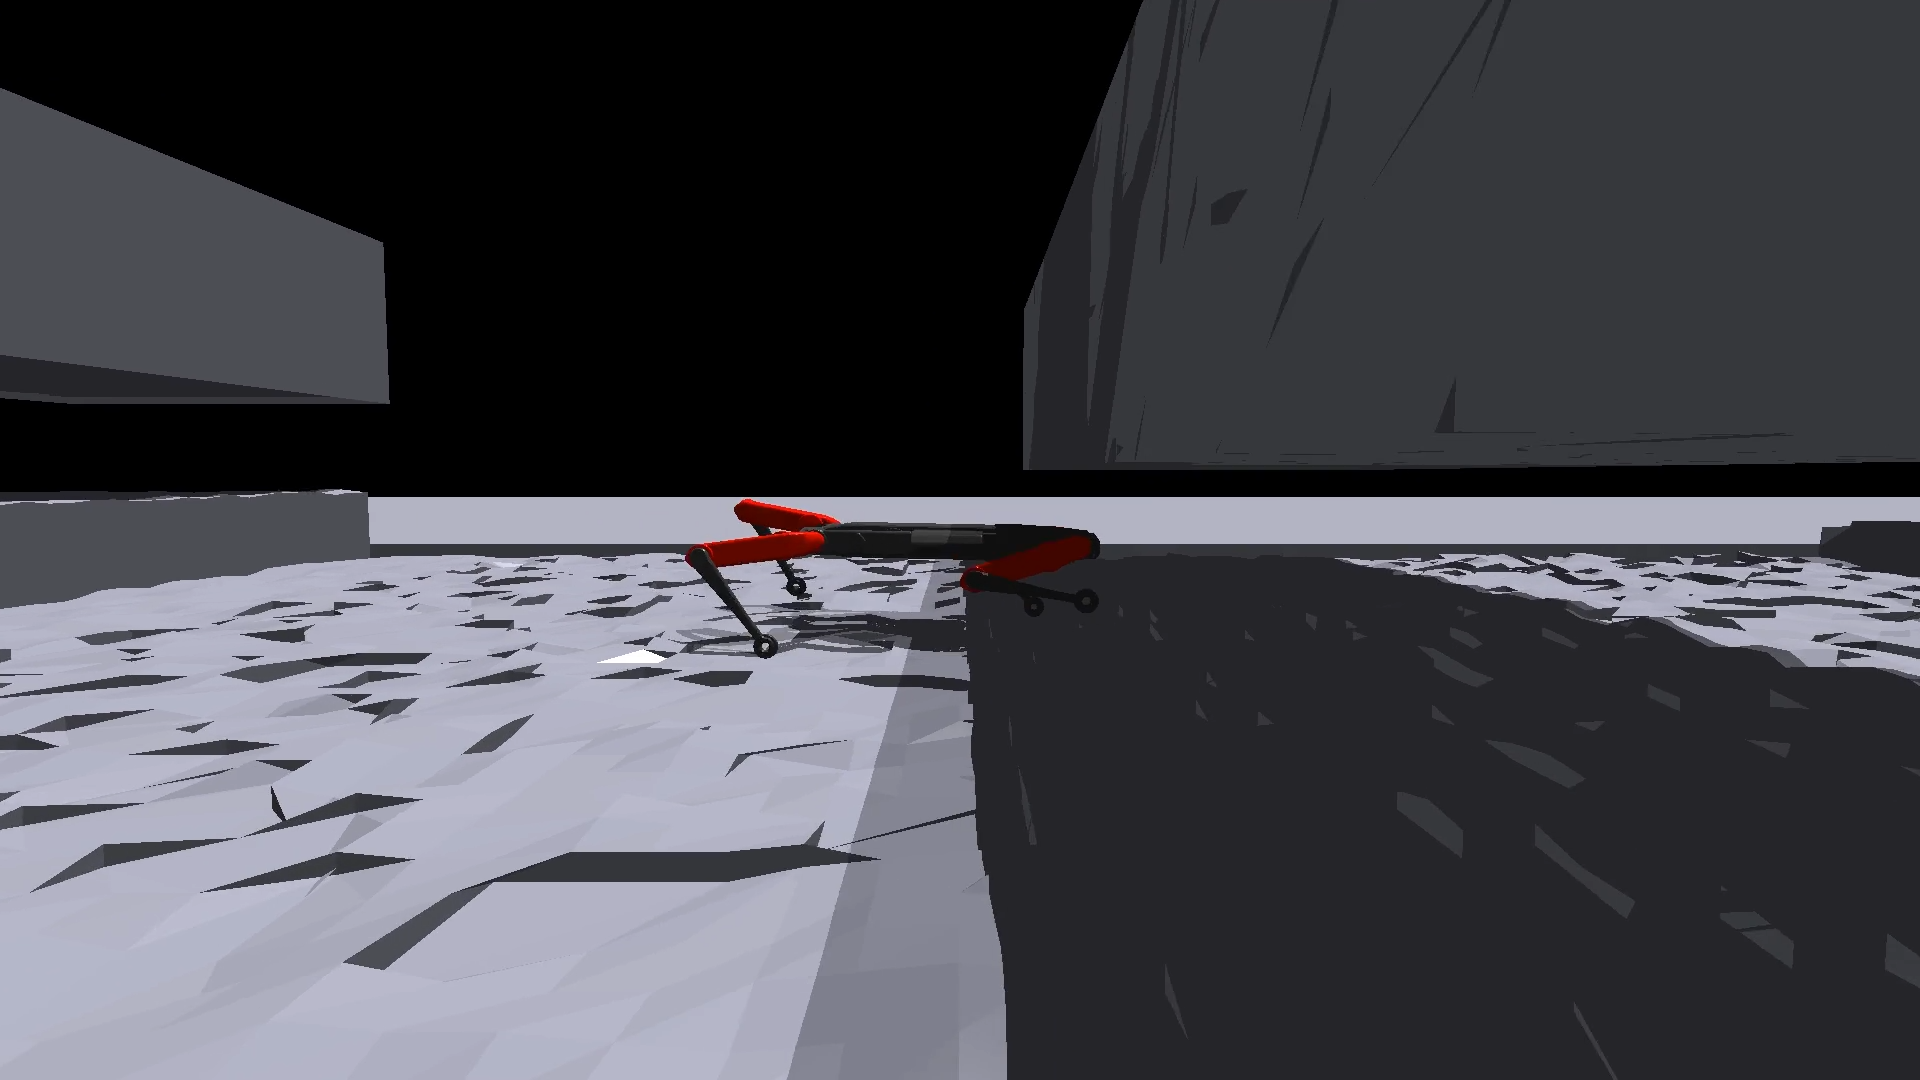
\includegraphics[width=\textwidth]{Assets/Terrains/crawl.png}
        \caption{Crawl}
        \label{fig:terrains:crawl}
    \end{subfigure}
    \hfill % this command adds space between the subfigures if needed
    \begin{subfigure}[b]{0.245\textwidth}
        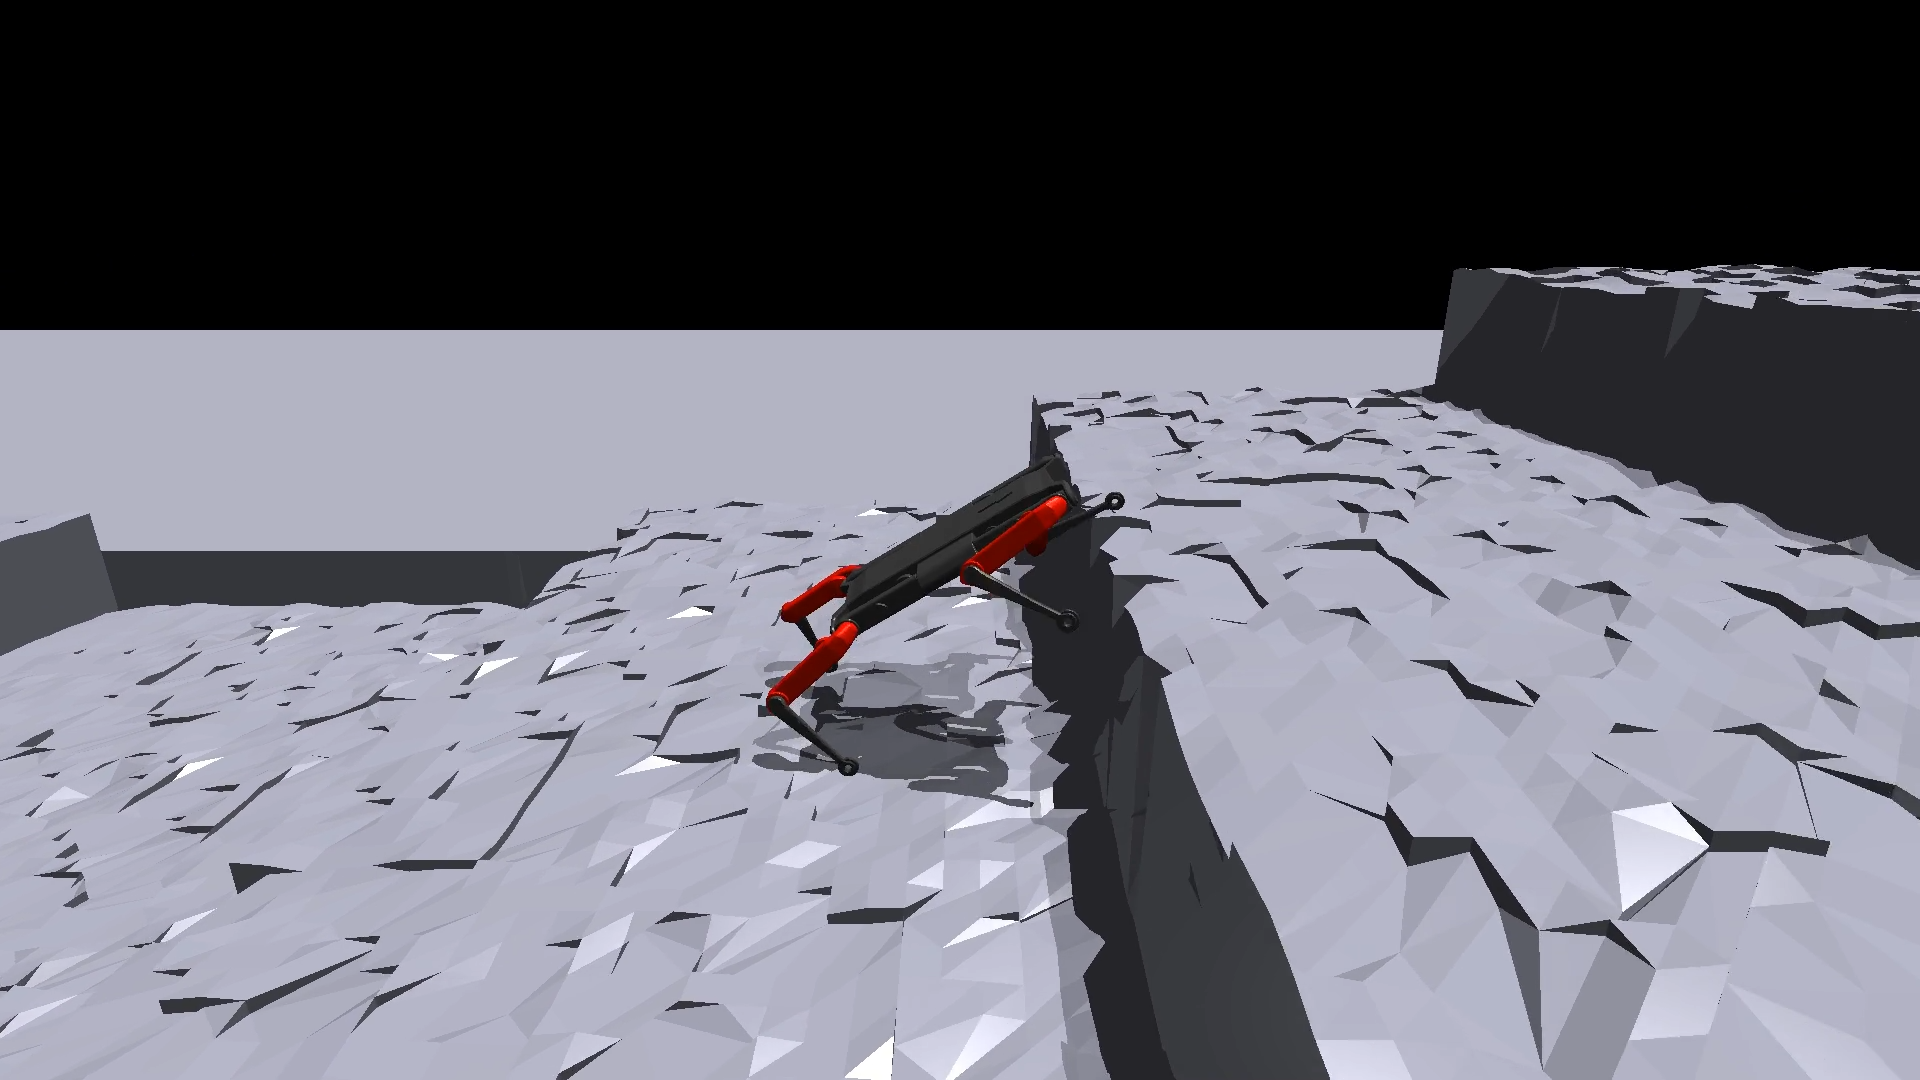
\includegraphics[width=\textwidth]{Assets/Terrains/steps.png}
        \caption{Climb}
        \label{fig:terrains:steps}
    \end{subfigure}
    \hfill
    \begin{subfigure}[b]{0.245\textwidth}
        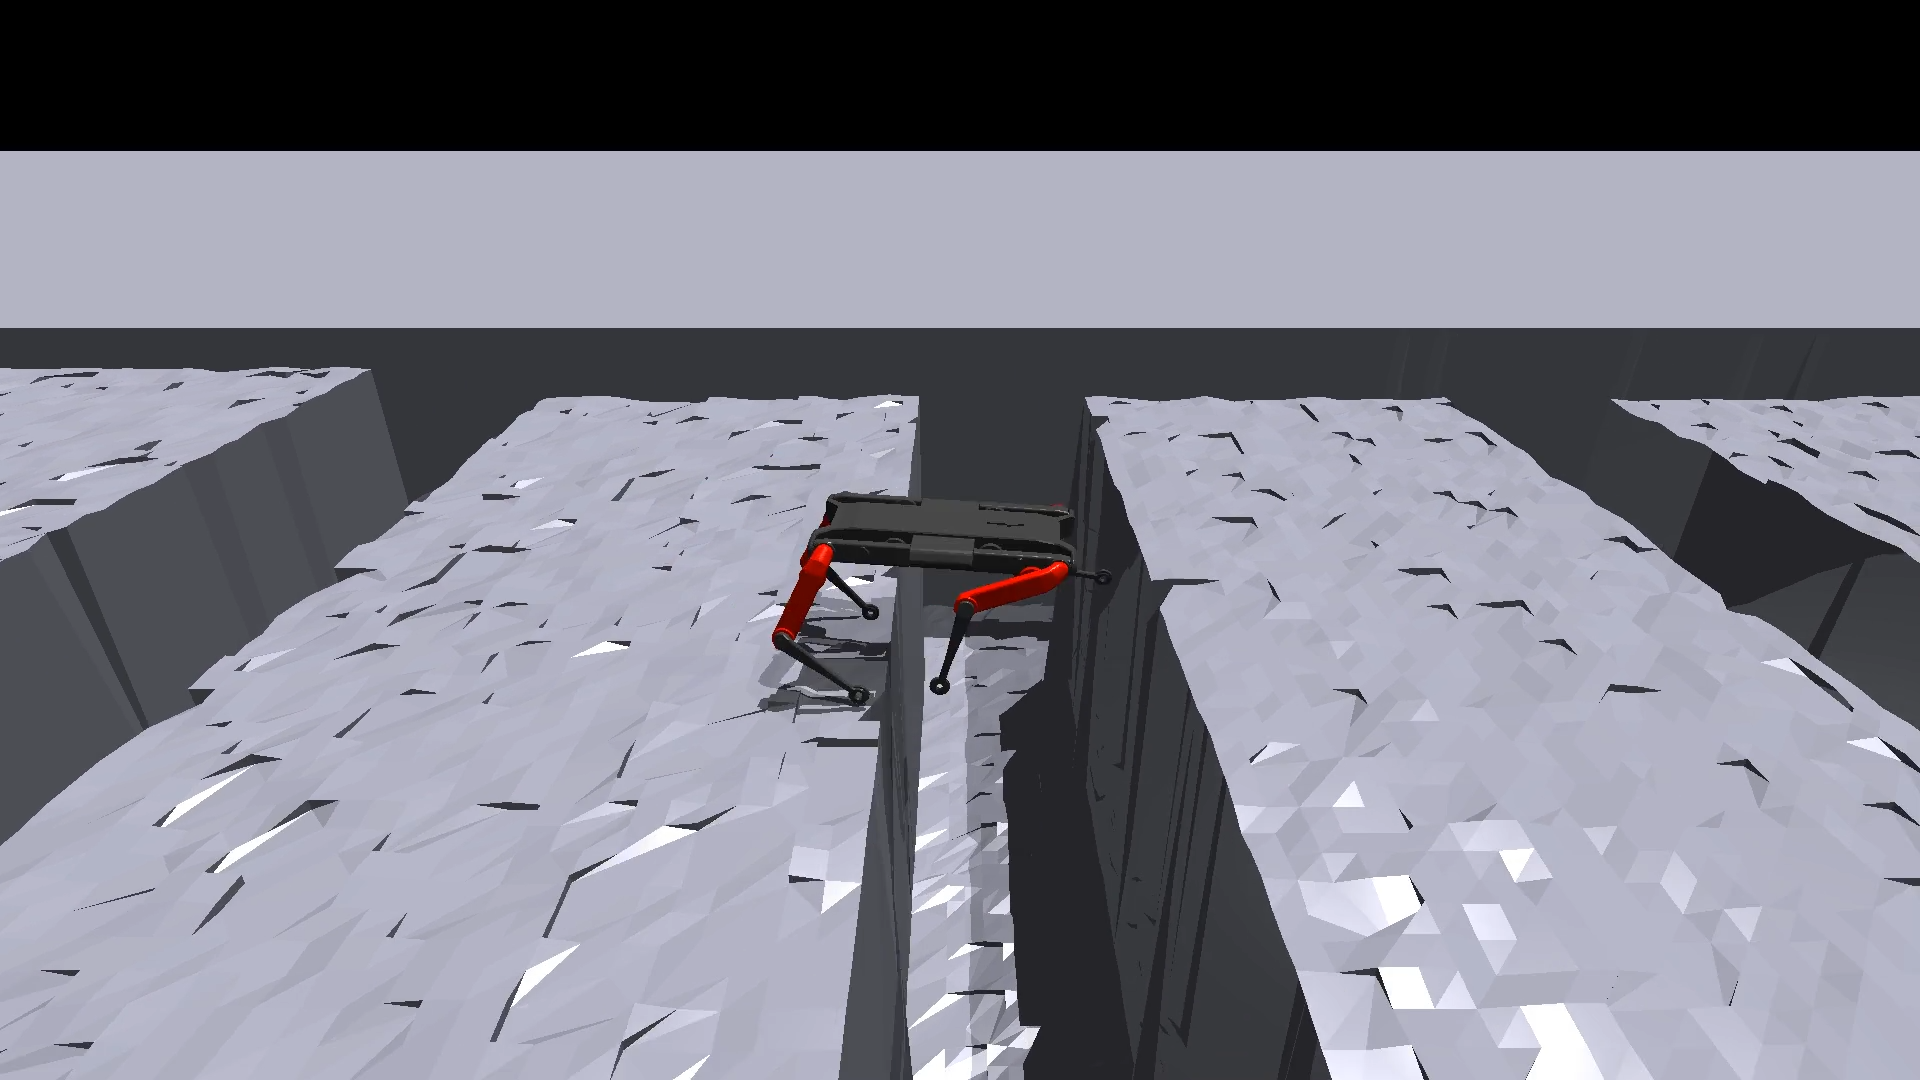
\includegraphics[width=\textwidth]{Assets/Terrains/gap.png}
        \caption{Leap}
        \label{fig:terrains:gap}
    \end{subfigure}
    \hfill
    \begin{subfigure}[b]{0.245\textwidth}
        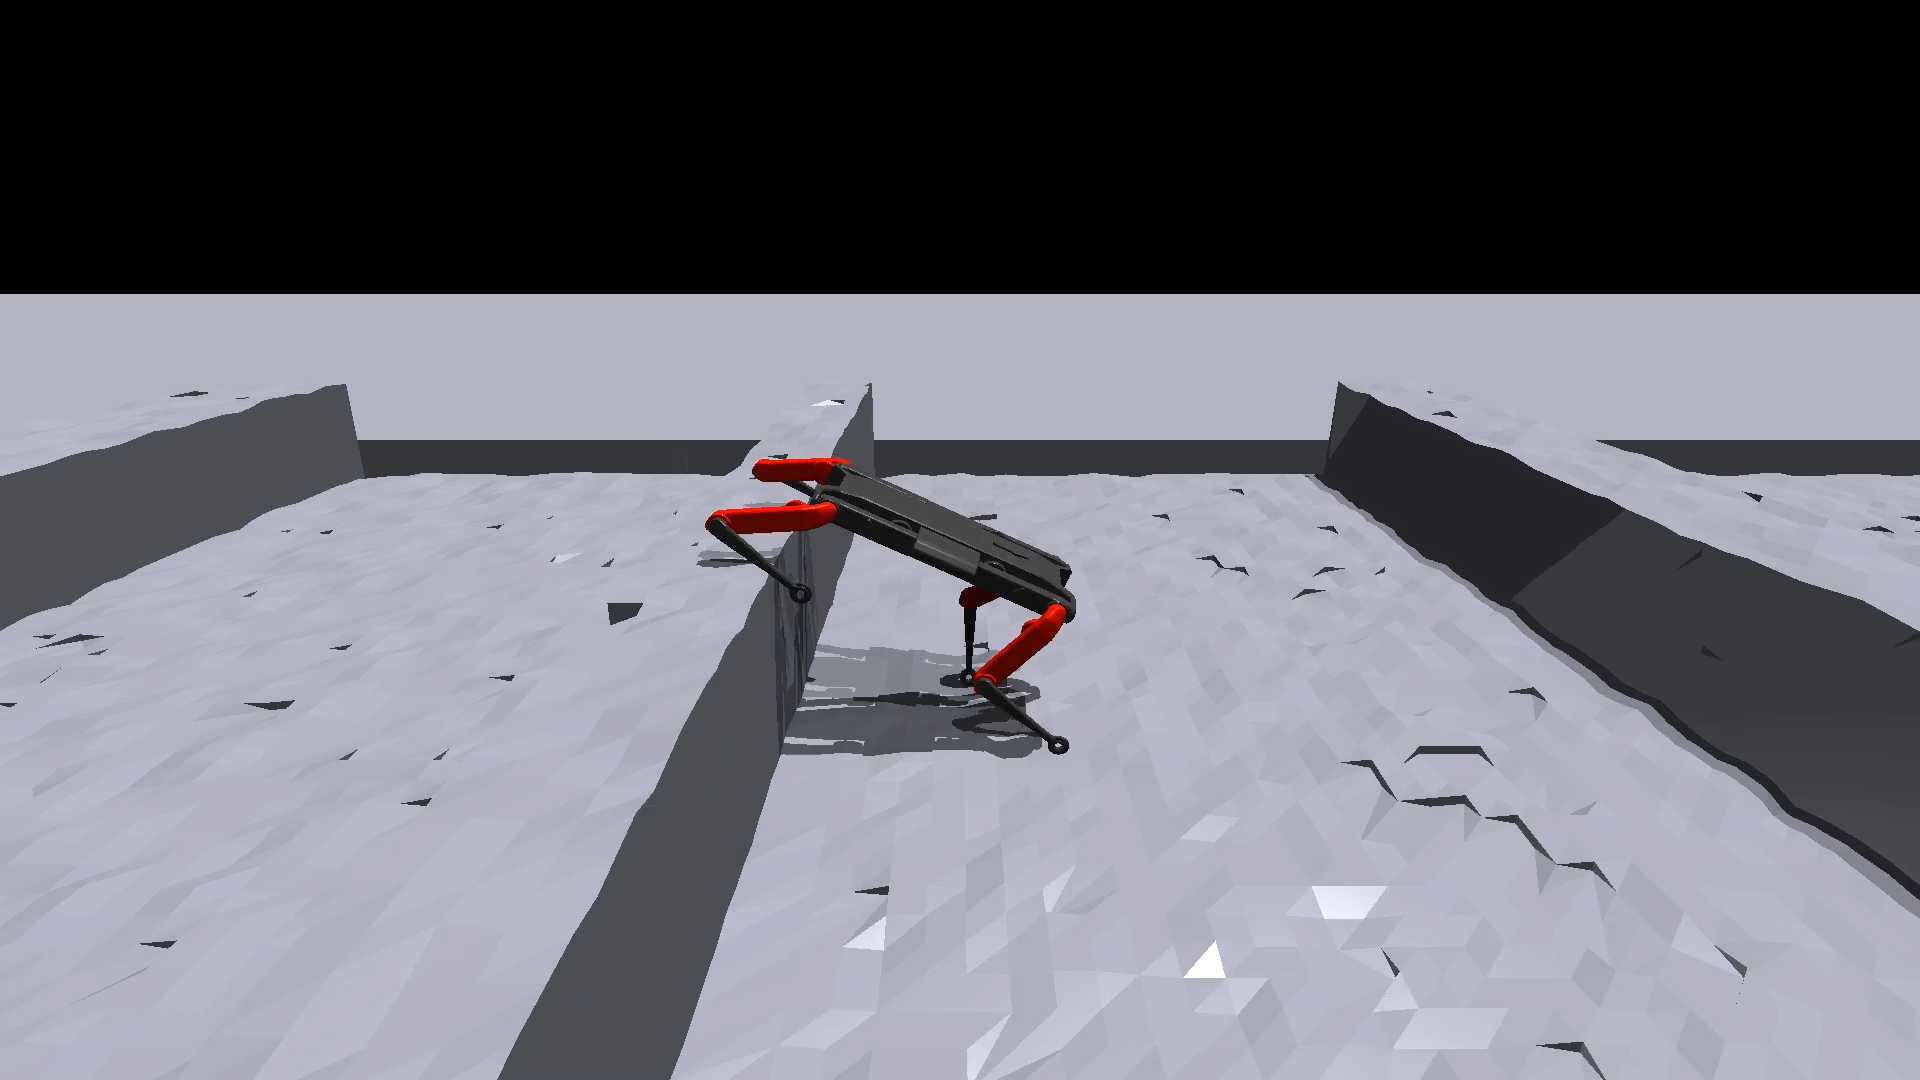
\includegraphics[width=\textwidth]{Assets/Terrains/hurdle.png}
        \caption{Hurdle}
        \label{fig:terrains:hurdle}
    \end{subfigure}
    \caption{Terrains used to train SoloParkour in simulation: the crawl parkour contains floating objects the robot must crawl under, the step and hurdle parkour contain obstacles for the robot to climb up and down, and the leap parkour contains gaps over which the robot must leap.}
    \label{fig:terrains}
    \vspace{-0.5cm}
\end{figure}

\paragraph{Terrains}
The policy is trained to traverse diverse challenging terrains in the IsaacGym simulator~\citep{makoviychuk2021isaac} to learn a variety of agile locomotion skills, as illustrated in Figure~\ref{fig:terrains}.
The focus of this work being on parkour, we consider learning locomotion skills such as walking, climbing, leaping, and crawling with four terrain types illustrated in Figure~\ref{fig:terrains}.
A single policy is jointly trained on a curriculum of variations of these terrains with increasing difficulty~\citep{rudin2022learning}.

%==============================================================================================



\subsection{Visual Policy Learning}

Ideally, we would like to train the policy from depth pixels to actions using deep RL in order to learn behaviors that best use the limited sensory inputs from the depth cameras.
However, directly training the vision policy end-to-end from scratch with RL is impractical, as depth images are costly to render in simulation.
An alternative approach is to first train a policy that has access to cheap-to-compute information only accessible in simulation about the terrain surrounding the robot, then distill the behaviors learned from this privileged information into a visual policy observing a history of depth images using imitation learning~\citep{agarwal2023legged, cheng2023parkour, zhuang2023robot}.
While the experimental setup can be chosen to reduce the distillation gap (e.g. by choosing specific sensors providing extensive observability), there is in general no guarantee that the learned behaviors will transfer well to the visual policy due to the observability gap between the privileged information and the visual sensors.
For instance, elevation maps may contain information about surfaces that are not visible from the camera inputs.
We then propose a generic solution mitigating these two problems.


\begin{figure}[t]
\centering
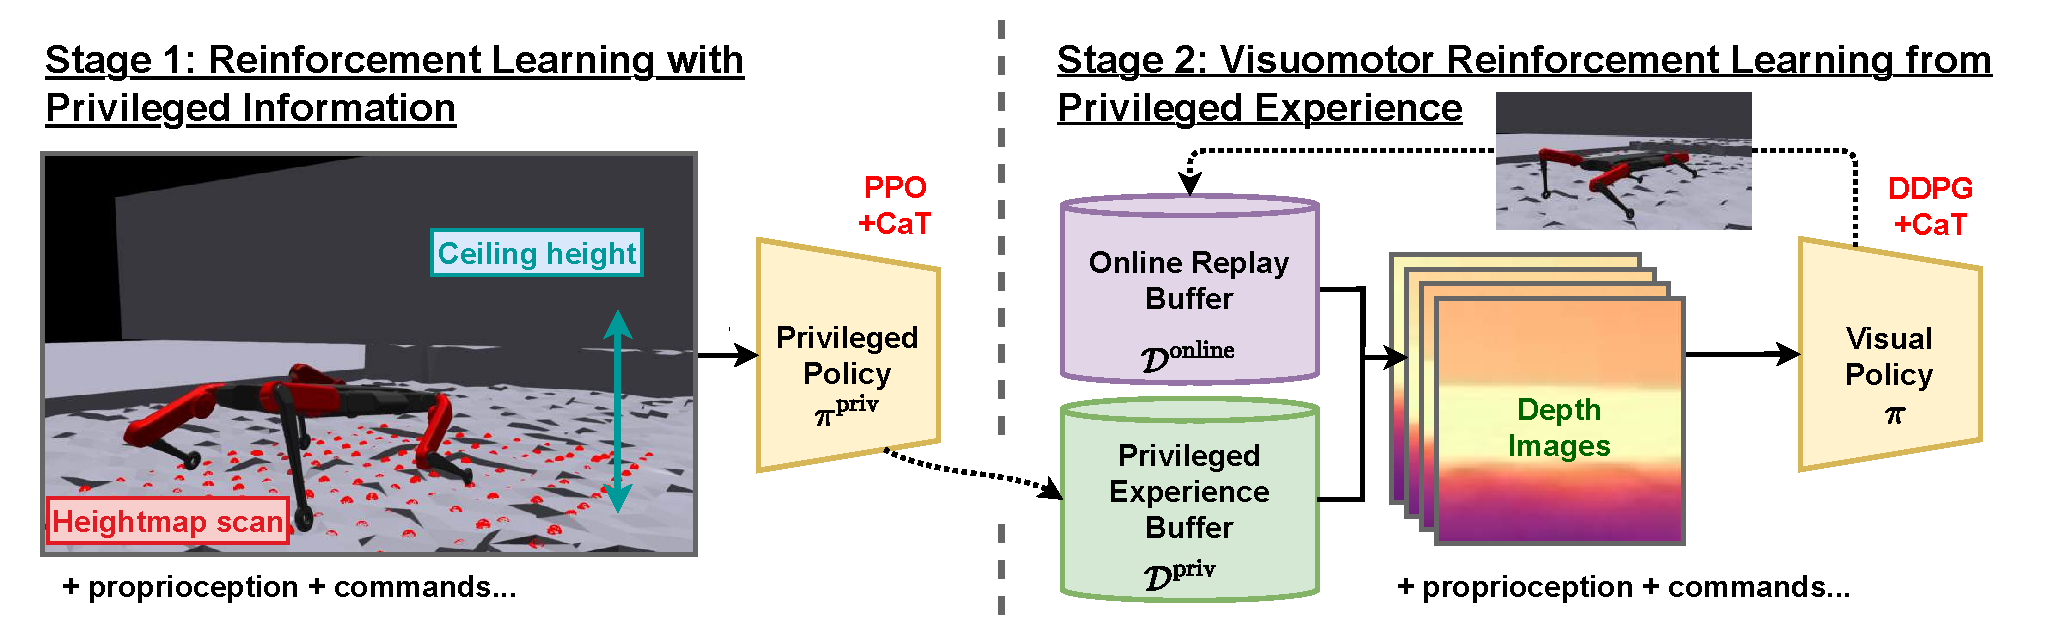
\includegraphics[width=1.0\linewidth]{Assets/Method.pdf}
\caption{SoloParkour leverages a two-stage RL approach to train visual locomotion policies in simulation. Stage 1: we train a privileged policy that observes a heightmap scan of its surroundings and the height of the nearby floating objects using PPO with Constraints as Terminations (CaT)~\citep{chane2024cat}. Stage 2: we train a policy from depth pixels using a variant of DDPG  with CaT that learns from a dataset of privileged experience collected using the Stage 1 policy.
}
\label{fig:method}
\vspace{-0.5cm}
\end{figure}

Our approach, SoloParkour, is illustrated in Figure~\ref{fig:method}.
Following prior works~\cite{agarwal2023legged,zhuang2023robot,cheng2023parkour}, we first learn a privileged policy that has access to cheap-to-compute information about the terrain surrounding the robot.
Unlike~\cite{agarwal2023legged,zhuang2023robot,cheng2023parkour}, we propose to use this privileged policy to warm-start the reinforcement learning of an end-to-end visual policy.
This way, we let the RL agent decide on the best behaviors given its limited sensory inputs while bypassing the computational complexity of training from depth images.

\paragraph{Stage 1: Privileged Policy Learning}
We first train a privileged policy $\pi^\text{priv}$ that has access to cheap-to-compute information about the terrain surrounding the robot.
In place of histories of depth images and proprioception, the robot observes the privileged state $s_t^\text{priv}$ that includes the current proprioceptive measures, velocity commands, and the previous action as well as a height-scan map of its surrounding and the ceiling height.
In crawl terrains, the ceiling height corresponds to the distance from the ground to a levitating block when such a block is near the robot.
In other terrains, or when no levitating blocks are nearby, the ceiling height is set to an arbitrarily high default value.
We found that this provides sufficient information about the terrain geometry to train the privileged policy for all the proposed terrain tracks.

The privileged policy is parameterized by a Multi-Layer Perceptron (MLP) trained using Proximal Policy Optimization~\citep{schulman2017proximal} (PPO), an on-policy RL method widely used in learning-based locomotion. We use CaT~\citep{chane2024cat} to enforce the constraints.

\paragraph{Stage 2: End-to-End Vision-Based RL from Privileged Experience}
To overcome the computational complexity of RL from pixels, we propose to adapt Reinforcement Learning with Prior Data~\citep{ball2023efficient} (RLPD) to transfer the experience from the privileged policy to visual locomotion and learn from depth images in a sample efficient manner.
We build on design principles from~\citep{smith2022legged, ball2023efficient, smith2023learning} and implement off-policy RL with a high update-to-data ratio.
Compared to on-policy approaches such as PPO, this minimizes the number of depth image rendering steps in simulation in favor of increased updates from the privileged and online experience.

More precisely, we employ a variant of Deep Deterministic Policy Gradient~\citep{lillicrap2015continuous} (DDPG) that uses two replay buffers: its online replay buffer $\mathcal{D}^\text{online}$ and a privileged experience buffer $\mathcal{D}^\text{priv}$. 
$\mathcal{D}^\text{priv}$ is constructed by employing the fully trained $\pi^\text{priv}$ from Stage 1 to generate demonstrations that include the depth modality $I^\text{depth}$.
During policy learning, batches of experiences are sampled in equal proportion from $\mathcal{D}^\text{online}$ and $\mathcal{D}^\text{priv}$ to train the policy $\pi$ and its Q-function.
We use REDQ~\citep{chen2021randomized} and Layer Normalization~\citep{ba2016layer} to stabilize Q-learning at high update-to-data ratio~\citep{smith2022walk, ball2023efficient, smith2023learning}.
Importantly, while the visual actor $\pi$ is trained end-to-end from a history of depth images, we found that training the critic from privileged state $s^\text{priv}_t$ rather than on the full state $s_t$ in an asymmetric actor-critic fashion~\citep{pinto2017asymmetric} was faster and more stable.
We incorporate CaT~\citep{chane2024cat} in an off-policy manner to learn visual locomotion that keeps satisfying the constraints.

The resulting RL algorithm is sample efficient enough to train our visual policies, parameterized by a ConvNet~\citep{lecun1998gradient} to process depth images individually, a Gated Recurrent Unit~\citep{chung2014empirical} to handle histories of observations, and an MLP head, with RL directly from pixels in simulation.

